\documentclass[preprint,superscriptaddress]{revtex4}
\usepackage{graphicx}
\usepackage{amsmath}
\begin{document}
\verb| |\\   % Seems to fix some latex bug
\special{papersize=8.5in,11in}

\begin{center}
{\large
\protect{\vspace{-2cm}}
Jefferson Lab PAC 44 Run-Group Proposal

\bf{The Transverse Nucleon, Single-Spin Asymmetry in
Exclusive Pion Electroproduction}\\[1ex]
}

DRAFT v0.1: \today\\[2ex]

SoLID Collaboration\\
\vspace{.15cm}

\end{center}

%\begin{abstract}

We propose to measure the transverse nucleon, single-spin asymmetry
$A_{UT}^{sin(\phi-\phi_s)}$ in the exclusive pion production
$\vec{n}(e,e'\pi^-)p$ reaction, during the transversely polarized $^3$He target
SIDIS experiment with SoLID.  This polarization observable has been noted as
being sensitive to the spin-flip generalized parton distribution (GPD)
$\tilde{E}$, and factorization studies have indicated that precocious scaling
is likely to set in at moderate $Q^2\sim 2-4$ GeV$^2$, as opposed to the
absolute cross section, where scaling is not expected until $Q^2>10$ GeV$^2$.
Furthermore, this observable has been noted as being important for the reliable
extraction of the charged pion form factor from pion electroproduction.  The
asymmetry data are projected to be of much higher quality than a pioneering
measurement by HERMES \cite{hermes10}.

This measurement is complementary to a proposal reviewed by PAC39 \cite{atpi39}
for the SHMS+HMS in Hall C.  The asymmetry that is most sensitive to
$\tilde{E}$ is the longitudinal photon, transverse nucleon, single-spin
asymmetry $A_L^{\perp}$ in exclusive charged pion electroproduction.  The
SHMS+HMS allow the L--T separation needed to reliably measure this quantity.
However, the limited detector acceptance and the error-magnification inherent
in an L--T separation necessitates the use of a next generation, externally
polarized, continuous flow, high luminosity $^3$He target based on a large
volume polarizer and compressor being developed at the University of New
Hampshire.

A wide $-t$ coverage is needed to obtain a good understanding of the asymmetry.
Thus, it has always been intended to complement the SHMS+HMS $A_L^{\perp}$
measurement with an unseparated $A_{UT}^{sin(\phi-\phi_s)}$ measurement using
a large solid angle detector.  The high luminosity capabilities of SoLID make
it well-suited for this measurement.  Since an L--T separation is not possible
with SoLID, the observed asymmetry is expected to be diluted by the ratio of
the longitudinal cross section to the unseparated cross section.  This was also
true for the pioneering HERMES measurements, which provided a valuable
constraint to models for the $\tilde{E}$ GPD.

%\end{abstract}

%\maketitle
\clearpage

\section{Scientific Justification}

{\bf{GH: This section is closely based on the Hall C proposal
    PR12-12-005.  Suggestions for modification are welcome!}}

\subsection{Generalized Parton Distributions and Contribution from the Pion
  Pole}

In recent years, much progress has been made in the theory of generalized
parton distributions (GPDs).  Unifying the concepts of parton distributions and
of hadronic form factors, they contain a wealth of information about how quarks
and gluons make up hadrons. The key difference between the usual parton
distributions and their generalized counterparts can be seen by representing
them in terms of the quark and gluon wavefunctions of the hadron.  While the
usual parton distributions are obtained from the squared hadron wavefunction
representing the probability to find a parton with specified polarization and
longitudinal momentum fraction $x$ in the fast moving hadron (Fig. 1a), GPDs
represent the interference of different wavefunctions, one where the parton has
momentum fraction $x+\xi$ and one where this fraction is $x-\xi$ (Fig. 1b).
GPDs thus correlate different parton configurations in the hadron at the
quantum mechanical level.  A special kinematic regime is probed in deep
exclusive meson production, where the initial hadron emits a quark-antiquark or
gluon pair (Fig. 1c).  This has no counterpart in the usual parton
distributions and carries information about $q\bar{q}$ and $gg$-components in
the hadron wavefunction.

\begin{figure}[hbtp!]
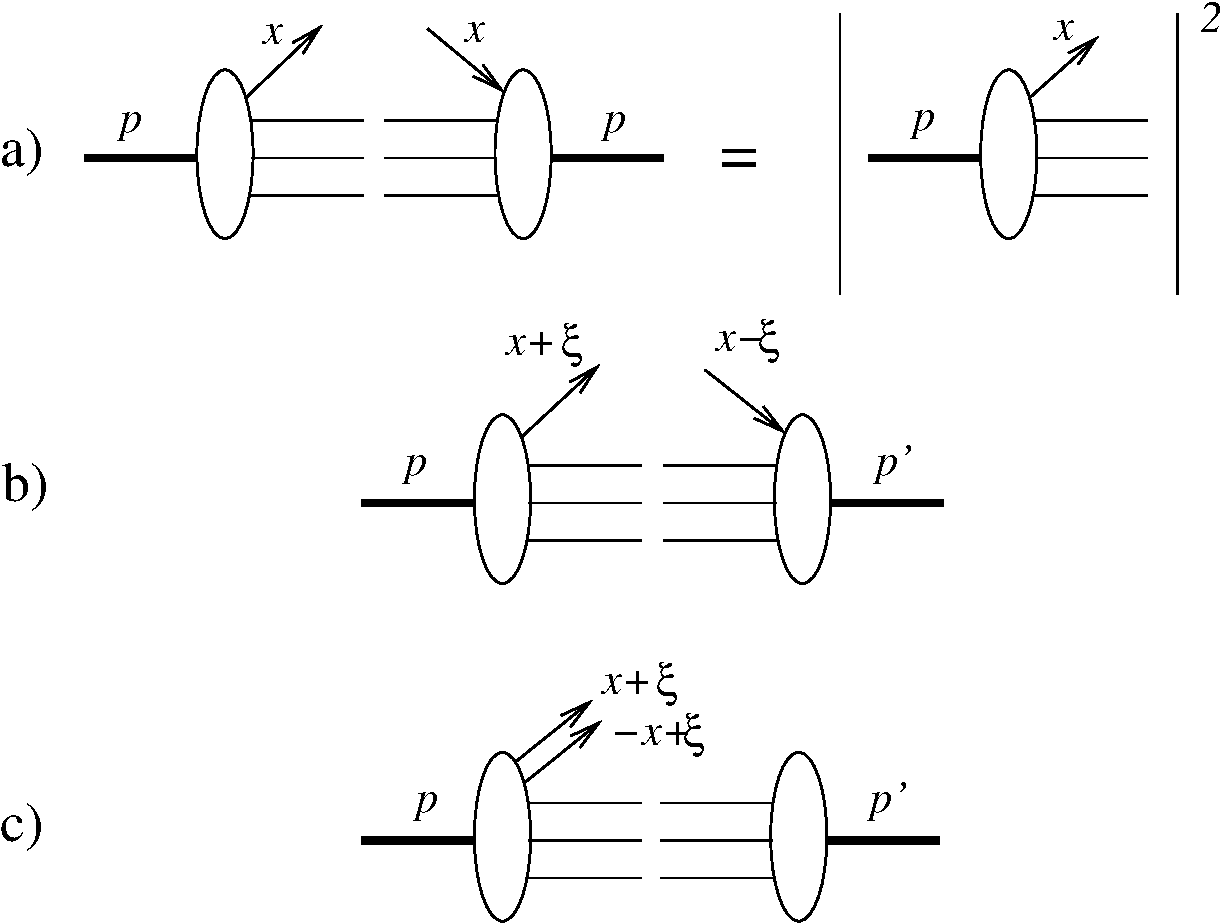
\includegraphics[height=6cm]{pdist_gpd_comparo.pdf}
\caption{\label{fig:pdis_gpd_comparo}
(a) Usual parton distribution, representing the probability to find a parton
with momentum fraction $x$ in the nucleon.
(b) GPD in the region where it represents the emission of a parton with
momentum fraction $x+\xi$ and its reabsorption with momentum fraction $x-\xi$.
(c) GPD in the region where it represents the emission of a quark-antiquark
pair, and has no counterpart in the usual parton distributions.
This figure has been adapted from Ref. \cite{Di00}.
}
\end{figure}

Apart from the momentum fraction variables $x$ and $\xi$, GPDs depend on the
four momentum transfer $t$.  This is an independent variable, because the
momenta $p$ and $p'$ may differ in either their longitudinal or transverse
components.  GPDs thus interrelate the longitudinal and transverse momentum
structure of partons within a fast moving hadron.

In order to access the physics contained within GPDs, one is restricted to the
hard scattering regime.  An important feature of hard scattering reactions is
the possibility to separate clearly the perturbative and nonperturbative stages
of the interaction.  Qualitatively speaking, the presence of a hard probe
allows one to create small size quark-antiquark and gluon configurations, whose
interactions are described by perturbative QCD (pQCD).  The non-perturbative
stage of the reaction describes how the hadron reacts to this configuration, or
how this probe is transformed into hadrons.  This separation is the so-called
factorization property of hard reactions.  Deep Exclusive Meson
electro-Production (DEMP) was first shown to be factorizable in
Ref. \cite{Co97}.  This factorization applies when the virtual photon is
longitudinally polarized, which is more probable to produce a small size
configuration compared to a transversely polarized photon.

GPDs are universal quantities and reflect the structure of the nucleon
independently of the reaction which probes the nucleon.  At leading twist-2
level, the nucleon structure information can  be parameterized in terms of four
quark chirality conserving GPDs, denoted $H$, $E$, $\tilde{H}$ and $\tilde{E}$.
$H$ and $E$ are summed over quark helicity, while $\tilde{H}$ and $\tilde{E}$
involve the difference between  left and right handed quarks.  $H$ and
$\tilde{H}$ conserve the helicity of the proton, while $E$ and $\tilde{E}$
allow for the possibility that the proton helicity is flipped.  Because quark
helicity is conserved in the hard scattering regime, the produced meson acts as
a helicity filter.  In particular, leading order QCD predicts that vector meson
production is sensitive only to the unpolarized GPDs, $H$ and $E$, whereas
pseudoscalar meson production is sensitive only to the polarized GPDs,
$\tilde{H}$ and $\tilde{E}$.  In contrast, deeply virtual Compton scattering
(DVCS) depends at the same time on both the polarized ($\tilde{H}$ and  
$\tilde{E}$) and the unpolarized ($H$ and $E$) GPDs.  This makes DEMP
reactions complementary to the DVCS process, as it
provides an additional tool to disentangle the different GPDs \cite{Go01}.

Besides coinciding with the parton distributions at vanishing momentum transfer
$\xi$, the GPDs have interesting links with other nucleon structure quantities.
Their first moments are related to the elastic form factors of the nucleon
through model-independent sum rules \cite{Ra00}:
\begin{eqnarray}
\sum_q e_q \int^{+1}_{-1} dx H^q(x,\xi,t) = F_1(t),\\
\sum_q e_q \int^{+1}_{-1} dx E^q(x,\xi,t) = F_2(t),\\
\sum_q e_q \int^{+1}_{-1} dx \tilde{H}^q(x,\xi,t) = G_A(t),\\
\sum_q e_q \int^{+1}_{-1} dx \tilde{E}^q(x,\xi,t) = G_P(t),
\end{eqnarray}
where $e_q$ is the charge of the relevant quark, $F_1(t)$, $F_2(t)$ are the
Dirac and Pauli elastic nucleon form factors, and $G_A(t)$, $G_P(t)$ are the
isovector axial and pseudoscalar nucleon form factors.  The $t$-dependence of
$G_A(t)$ is poorly known, and although $G_P(t)$ is an important quantity, it
remains highly uncertain because it is negligible at the momentum transfer of
$\beta$-decay\cite{Th01}.  Because of partial conservation of the axial current
(PCAC), $G_P(t)$ alone
receives contributions from $J^{PG}=0^{--}$ states\cite{Ma69}, which are the
quantum numbers of the pion, and so $\tilde{E}$ contains an important pion pole
contribution (Fig. 2a).

\begin{figure}[hbtp!]
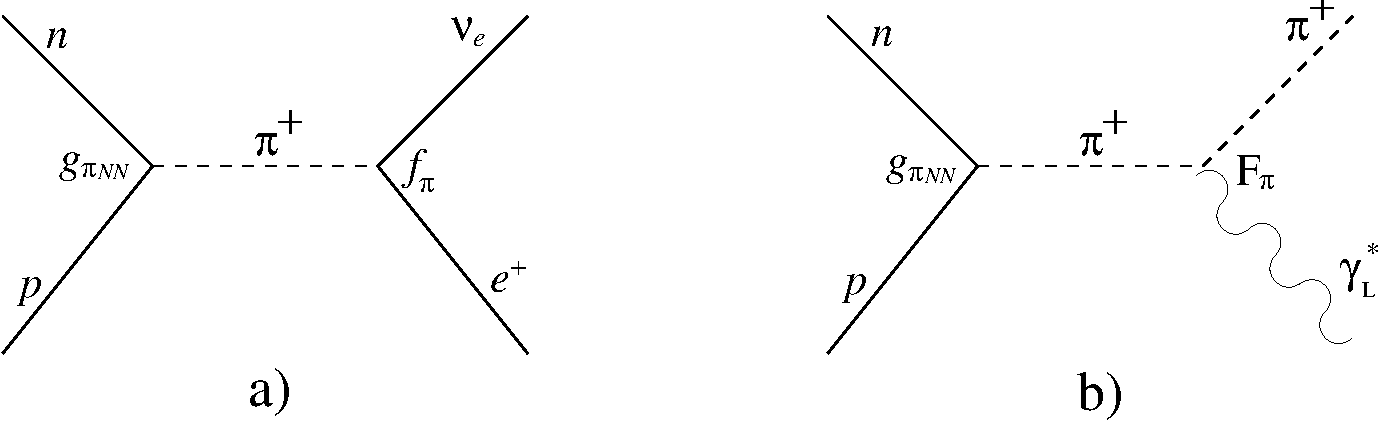
\includegraphics[height=4cm]{PCAC_pion_pole.pdf}
\caption{\label{fig:PCAC_pion_pole}
(a) Pion pole contribution to $G_P(t)$, and hence to $\tilde{E}$.
(b) Pion pole contribution to meson electroproduction at low $-t$.
}
\end{figure}

Accordingly, Refs. \cite{Pe00,Be01} have adopted the pion pole-dominated
ansatz
\begin{equation}
\tilde{E}^{ud}(x,\xi,t) = F_{\pi}(t)\frac{\theta (\xi>|x|)}{2\xi
}\phi_{\pi}(\frac{x+\xi}{2\xi}),
\end{equation}
where $F_{\pi}(t)$ is the pion electromagnetic form factor, and $\phi_{\pi}$ is
the pion distribution amplitude.

$\tilde{E}$ cannot be related to already known parton distributions,
and so experimental information about $\tilde{E}$ via DEMP 
can provide new information on nucleon structure which is
unlikely to be available from any other source.

\begin{figure}[hbt!]
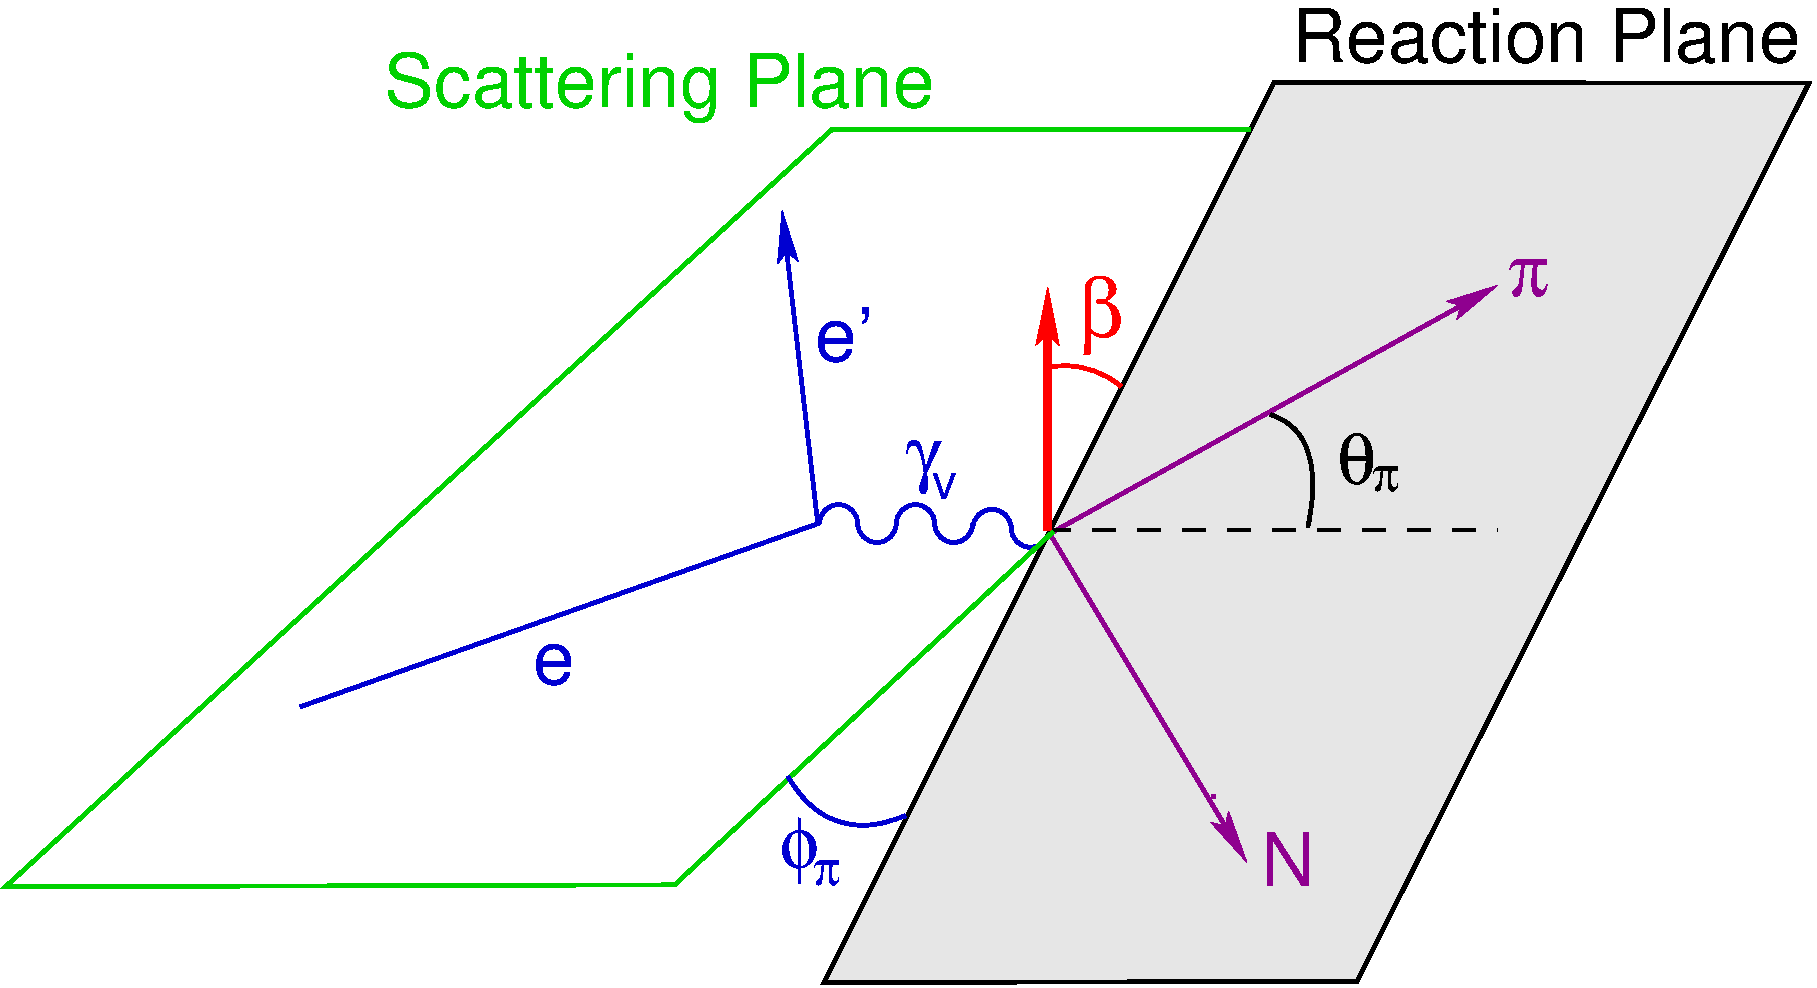
\includegraphics[height=6cm]{atpi_planes.pdf}
\caption{\label{fig:planes}
Scattering and hadronic reaction planes for exclusive $\vec{N}(e,e'\pi)N'$.
$\beta$ is the angle between the target nucleon polarization vector and the
reaction plane.  Some works alternatively label this angle as $(\phi-\phi_s)$.
}
\end{figure}

\subsection{Single spin asymmetry in exclusive pion electroproduction}

Frankfurt et al. \cite{Fr99} have considered a specific polarization observable
which is the most sensitive observable to probe the spin-flip $\tilde{E}$.
This variable is the single-spin asymmetry for exclusive charged pion
production, $\vec{p}(e,e'\pi^+)n$ or $\vec{n}(e,e'\pi^-)p$, from a transversely
polarized nucleon target, and is defined \cite{Be01} as
\begin{equation} \label{eqn:asy}
A_L^{\perp}=(\int^{\pi}_0 d\beta \frac{d\sigma^{\pi}_L}{d\beta} -
\int^{2\pi}_{\pi} d\beta \frac{d\sigma^{\pi}_L}{d\beta})
(\int^{2\pi}_0 d\beta \frac{d\sigma^{\pi}_L}{d\beta})^{-1},
\end{equation}
where $d\sigma^{\pi}_L$ is the exclusive charged pion electroproduction cross
section using longitudinally polarized photons and $\beta$ is the angle between
the nucleon polarization vector and the reaction plane (Fig.~\ref{fig:planes}).  
Frankfurt et al. \cite{Fr99} have shown that this asymmetry must vanish if
$\tilde{E}$ is zero.  If $\tilde{E}$ is not zero, the asymmetry will display a
sin$\beta$ dependence.  Their predicted asymmetry using the $\tilde{E}$ ansatz
from Ref. \cite{Va99} is shown in Fig. \ref{fig:frankfurt_atpi}.  This
calculation is $Q^2$-independent, depending only on how well the soft
contributions cancel in the asymmetry.

\begin{figure}[hbt!]
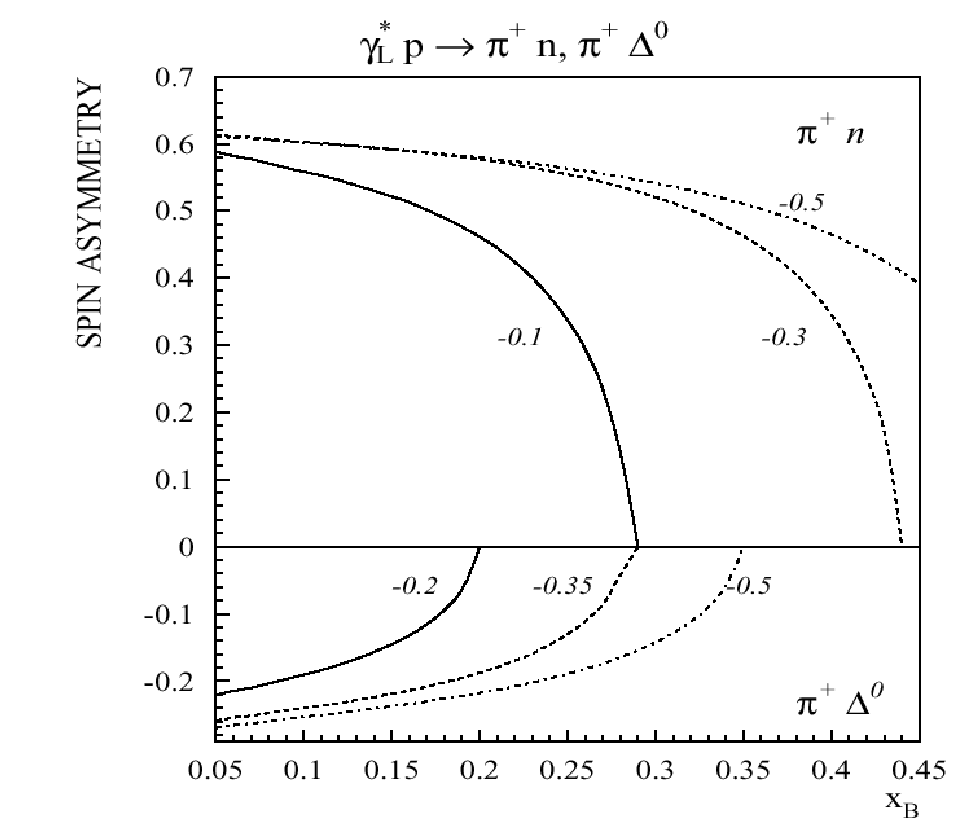
\includegraphics[height=7cm]{frankfurt_atpi.pdf}
\caption{\label{fig:frankfurt_atpi}
Transverse single-spin asymmetry for the longitudinal electroproduction of
$\pi^+n$ and $\pi^+\Delta^0$ at different values of $t$ [indicated on the
curves in GeV$^2$].  The asymmetry drops to zero at the parallel kinematic
limit, which is different for each $t$ value, because the definition of
$\beta$ is ill-defined at this point.  This figure is taken from
Ref. \protect{\cite{Fr00}}.
}
\end{figure}

It seems likely that a precocious factorization of the meson production
amplitude into three parts -- the overlap integral between the photon and pion
wave functions, the hard interaction, and the GPD -- will lead to a precocious
scaling of $A_L^{\perp}$ as a function of $Q^2$ at moderate $Q^2\sim 2-4$
GeV$^2$ \cite{Fr99}.  This precocious scaling arises from the fact that higher
order corrections, which are expected to be significant at low $Q^2$, will
likely cancel when one examines the ratio of two longitudinal observables.  In
contrast, the onset of scaling for the absolute cross section is only expected
for much larger values of $Q^2>10$ GeV$^2$.

\begin{figure}[hbt!]
\begin{center}
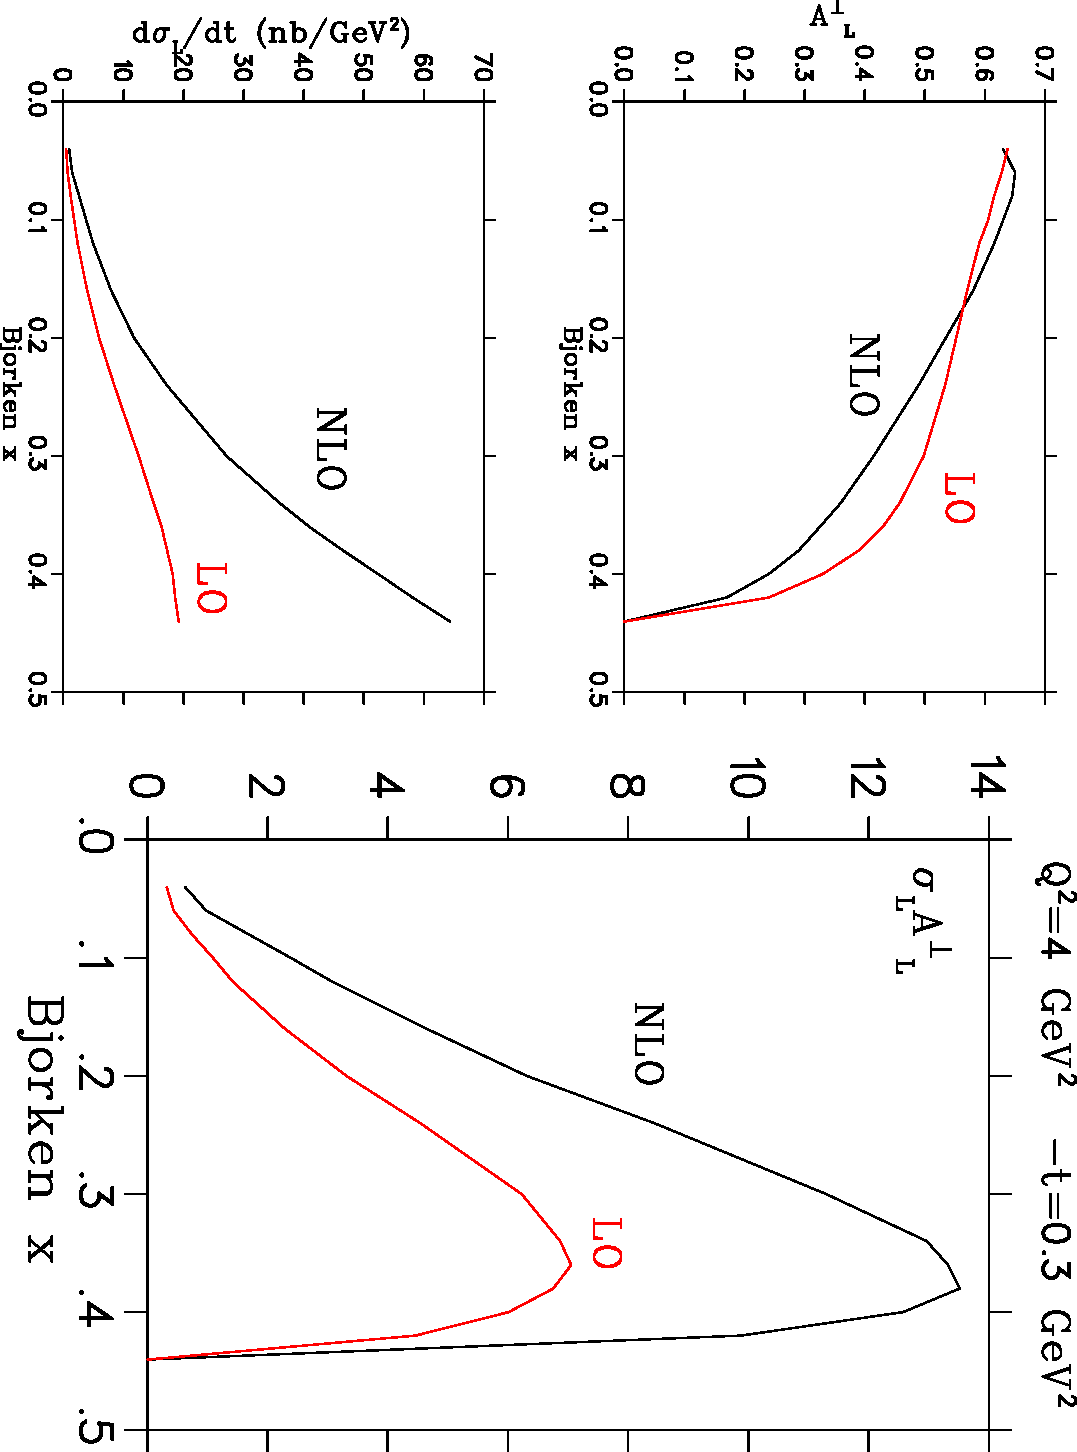
\includegraphics[height=10cm,angle=90.]{belitsky.pdf}
\caption{\label{fig:belitsky_atpi}
Calculation of the longitudinal photon transverse nucleon spin asymmetry
including twist-four corrections by A. Belitsky \cite{belitsky} at $-t=0.3$
GeV$^2$, $Q^2$=4 GeV$^2$.  The red curves are the leading order calculation,
while the black curves have twist-four power effects taken into account.  While
the cross section is very sensitive to these corrections, the transverse spin
asymmetry is stable.  The figure of merit $\sigma_L A_L^{\perp}$ maximum at
$x_B=0.37$ corresponds to particle angles and momenta similar to those proposed
here.}
\end{center}
\end{figure}

This point is made clear in Fig. \ref{fig:belitsky_atpi}.  This figure shows
renormalon model calculations \cite{belitsky} of both the asymmetry and the
longitudinal cross section at $Q^2=4$ GeV$^2$.  While the magnitude of the
cross section changes significantly when taking into account the twist-four
corrections, $A_L^{\perp}$ is essentially insensitive to them and displays the
expected precocious scaling.  The relatively low value of $Q^2$ for the
expected onset of precocious scaling is important, because it will be
experimentally accessible after the Jefferson Lab 12 GeV upgrade.  This places
$A_L^{\perp}$ among the most important GPD measurements that can be made in the
meson scalar.  If precocious scaling cannot be experimentally demonstrated in
this ratio of two cross sections, then it may not be possible to determine
GPDs from DEMP data.

Refs. \cite{Go01} and \cite{Fr00} also point out that the study of the
transverse target single-spin asymmetry versus $t$ is important for the
reliable extraction of the pion form factor from electroproduction experiments
(Fig. 2b).  Investigations of hard exclusive $\pi^+$ electroproduction using a
pQCD factorization model \cite{Ma99,Ca90} find that at $x_B=0.3$ and
$-t=-t_{min}$, the pion pole contributes about 80\% of the longitudinal cross
section.  Since the longitudinal photon transverse single-spin asymmetry is an
interference between
pseudoscalar and pseudovector contributions, its measurement would help
constrain the non-pole pseudovector contribution, and so assist the more
reliable extraction of the pion form factor.  The upper $Q^2=6$ GeV$^2$ limit
of the approved pion form factor measurements in the JLab 12 GeV program
\cite{12GeV} is dictated primarily by the requirement $-t_{min}<0.2$ GeV$^2$,
to keep non-pion pole contributions to $\sigma_L$ at an acceptable level
\cite{Ca90}.  Transverse target single-spin asymmetry studies versus $t$ may
eventually allow, with theoretical input, the use of somewhat larger $-t$ data
for pion form factor measurements, ultimately extending the $Q^2$-reach of pion
form factor data acquired with JLab 12 GeV beam.  Thus, measurements of
the transverse single-spin asymmetry are a logical step in the support of the
pion form factor program.

\subsection{The Complementarity of Separated and Unseparated Asymmetry
  Measurements}

It has not yet been possible to perform an experiment to measure $A_L^{\perp}$.
The conflicting experimental requirements of transversely polarized target,
high luminosity, L--T separation, and closely controlled systematic
uncertainty, make this an exceptionally challenging observable to measure.  The
SHMS+HMS is the only facility with the necessary resolution and systematic
error control to allow a measurement of $A_L^{\perp}$.  However, the beamtime
required to do a good measurement with current polarized target technology is
in the range of 10$^3$ days.  To minimize the beamtime required, PR12-12-005
proposed the use of a next generation, externally polarized, continuous flow,
high luminosity $^3$He target based on a large volume polarizer and compressor
developed at the University of New Hampshire \cite{atpi39}.  The science case
for this measurement was favorably reviewed by PAC39, and they encouraged the
continued development of the target technology.  Although the New Hampshire
group is making continued progress on the development of the target, there is
no timeline for its actual implementation at Jefferson Lab.

The most closely related measurement, of the transverse single-spin asymmetry
in exclusive $\pi^+$ electroproduction without an L--T separation, was
published by the HERMES Collaboration in 2010 \cite{hermes10}.  Their data were
obtained for average values of $\langle x_B \rangle =0.13$, $\langle Q^2 \rangle
=2.38$ GeV$^2$ and $\langle t' \rangle = -0.46$ GeV$^2$, subject to the
criterion $W^2>10$ GeV$^2$.  The six Fourier amplitudes in terms of the
azimuthal angles $\phi$, $\phi_s$ of the pion-momentum and proton-polarization
vectors relative to the lepton scattering plane were determined.  Of these, at
leading twist only the $\sin(\phi-\phi_s)_{UT}$ Fourier amplitude receives a
contribution from longitudinal photons.  If one assumes that longitudinal
contributions dominate, these $A_{UT}^{sin(\phi-\phi_s)}$ values can be
compared to GPD models for $\tilde{E}$, $\tilde{H}$.

\begin{figure}[hbt!]
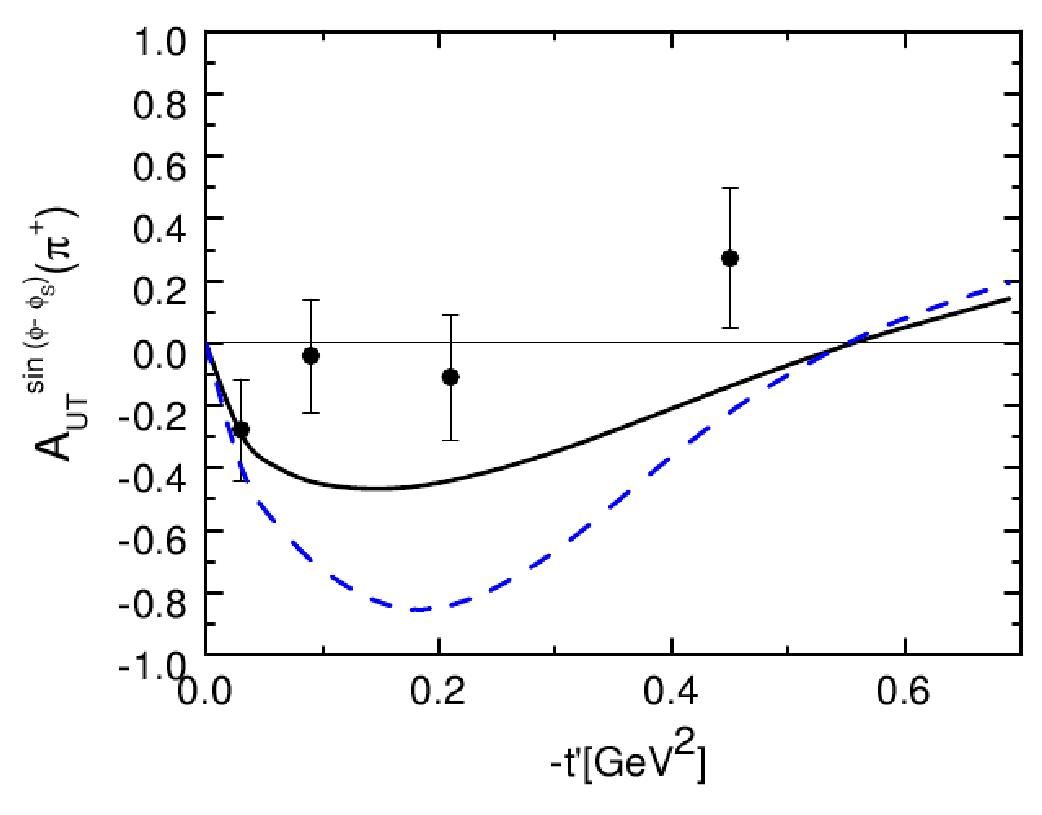
\includegraphics[height=7cm]{hermes_Aut.pdf}
\caption{\label{fig:hermes_aut}
Predictions by Goloskokov and Kroll for the sin$(\phi-\phi_s)$ moment of
$A_{UT}$ in the handbag approach, in comparison to the data from HERMES at
$Q^2=2.45$ GeV$^2$, $W=3.99$ GeV.  The independent variable is
$-t'=|t-t_{min}|$.  Dashed line: contribution from longitudinal photons only.
Solid line: full calculation including both transverse and longitudinal
photons.  This figure is taken from Ref. \protect{\cite{Go10}}.}
\end{figure}

Because transverse photon amplitudes are suppressed by $1/Q$, at very high
$Q^2$ it is safe to assume that all observed meson production is due to
longitudinal photons.  At the lower $Q^2$ typical of the JLab and HERMES
programs, however, this is not the case.  Calculations by Goloskokov and Kroll
\cite{Go10} indicate much of the unseparated cross section measured by HERMES
\cite{hermes10} is due to contributions from transversely polarized photons.
In addition, there are contributions to $A_{UT}^{sin(\phi-\phi_s)}$ from the
interference between two amplitudes, both for longitudinal photons, as well as
transverse photons~\cite{Di05}.  As indicated in Fig. \ref{fig:hermes_aut}, the
contribution from transverse photons tends to make the asymmetry smaller.  At
the HERMES kinematics, the dilution caused by transverse photons is about
50\%.

\begin{figure}[hbt!]
\begin{center}
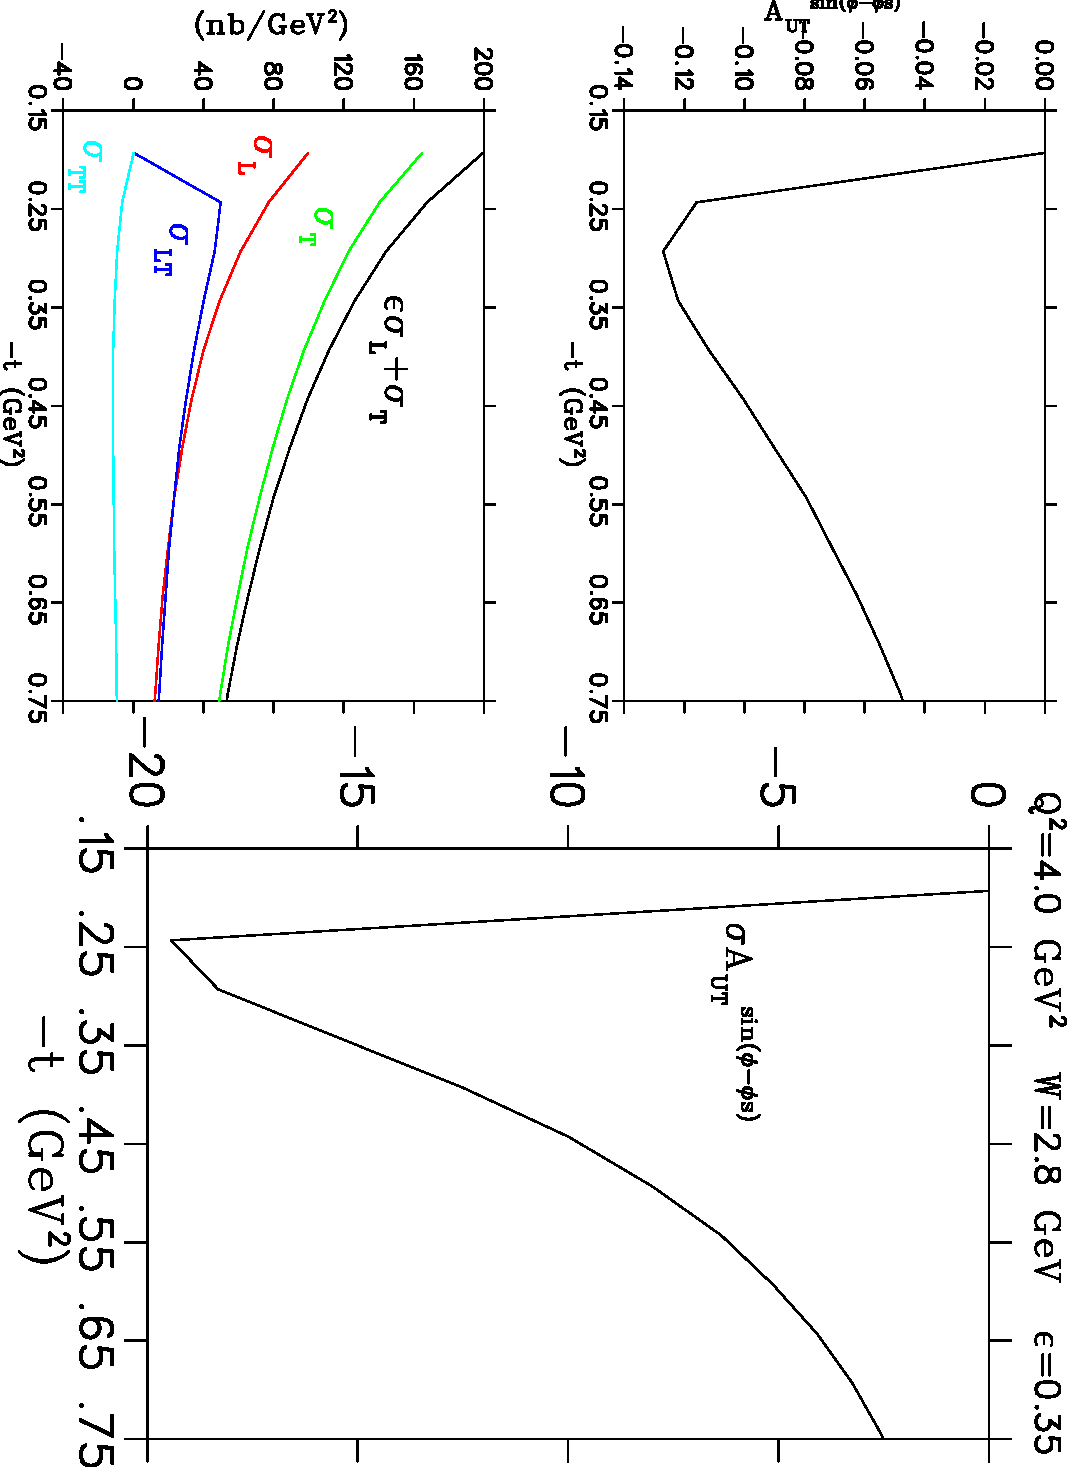
\includegraphics[height=10cm,angle=90.]{goloskokov_qsq4p0_w2p8.pdf}
\caption{\label{fig:golo_aut}
Calculation of the cross section components and sin$(\phi-\phi_s)$ moment of
the transverse nucleon spin asymmetry $A_{UT}$ in the handbag approach by
Goloskokov and Kroll \cite{GoPC} for kinematics similar to those in
Fig. \ref{fig:belitsky_atpi}.  $x_B=0.365$ for the kinematics in this
figure.}
\end{center}
\end{figure}

A run-group proposal concurrent with the SoLID transversely polarized $^3$He
SIDIS experiment allows for an unseparated asymmetry measurement to be obtained
on a sooner timescale than the Hall C measurement.  In comparison to the HERMES
measurement, the experiment proposed here will probe higher $Q^2$ and $x_B$,
with much smaller statistical errors over a wider range of $-t$.
SoLID will allow the first measurement for $Q^2>4$ GeV$^2$, where GPD-based
calculations are expected to apply.  Thus, the measurements should be more
readily interpretable than those from HERMES.  Similar measurements using
CLAS-12 and a transversely polarized $^1$H target have been discussed
previously \cite{clas}, but this measurement will allow for smaller statistical
uncertainties, due to SoLID's higher luminosity capabilities.

Handbag model calculations by Goloskokov and Kroll \cite{GoPC} shed further
light on the expected asymmetry dilution.  The lower left panel of
Fig. \ref{fig:golo_aut} shows their predictions for the cross section
components in exclusive charged pion production.  Although their calculations
tend to underestimate the $\sigma_L$ values measured in the JLab $F_{\pi}-2$
experiment \cite{Fpi2}, their model is in reasonable agreement with the
unseparated cross sections \cite{Go10}.  They predict significant transverse
contributions for JLab kinematics.  A comparison of the unseparated asymmetry
at $-t=0.3$ GeV$^2$, $x_B=0.365$ in Fig. \ref{fig:golo_aut} with the separated
longitudinal asymmetry at the same values of $x_B$, $-t$ in
Fig. \ref{fig:belitsky_atpi} indicates a substantial dilution of the
unseparated asymmetry due to transverse photon contributions, similar to that
observed in Fig. \ref{fig:hermes_aut}.

In addition to allowing a measurement at $Q^2>4$ GeV$^2$, a measurement by
SoLID of $A_{UT}^{sin(\phi-\phi_s)}$ will cover a fairly large range of $-t$,
allowing the asymmetry to be mapped over its full range with good statistical
uncertainties -- from its required zero-value in parallel kinematics, through
its maximum, and then back to near-zero as $\sigma_T$ dominates $\sigma_L$ at
larger $-t$.  The shape of the asymmetry curve versus $-t$, as well as its
maximum value, are critical information for comparison to GPD-based models.  At
a later date, the New Hampshire polarized target might enable a measurement of
$A_L^{\perp}$ in Hall C.  Although undiluted, the error-magnification
inherent in an L--T separation will make for larger uncertainties.  The
comparison of the maxima and $t$-dependences of both measurements will provide
complementary data needed to extract $\tilde{E}$ information and better
understand non-pole contributions complicating the extraction of the pion form
factor from electroproduction data.

\section{Experimental Method}

{\bf{GH: This section is a place-holder for new text that needs to be
    written.}}

Experimentally, the angle between the target polarization and the reaction
plane, $\beta$, and the angle between the scattering and reaction planes,
$\phi$, are not independent.  If the target polarization is at some angle,
$\phi_s$, relative to the scattering plane, then $\beta = \phi_s-\phi$.  For
the experimental set--up that will be discussed here, $\phi_s$ is relatively
constant, so it will be useful to re--express the above cross sections in terms
of $\beta$ and $\phi_s$.  The polarized nucleon cross section then becomes:
\begin{multline}\label{eqn:sigtarg}
\sigma_t =  - P_\perp \sin \beta \left[\sigma^y_{TT}+ 2\epsilon \; 
  \sigma^y_L \right] \\
- P_\perp \sin \beta \left[\epsilon (\cos 2\phi_s \cos 2\beta + 
  \sin 2\phi_s \sin 2\beta) \; \sigma^y_{TT'} \right]\\
- P_\perp \sin \beta \left[\sqrt{2\epsilon(1+\epsilon)}(\cos \phi_s \cos \beta 
  + \sin \phi_s \sin \beta) \; \sigma^y_{LT}\right] \\
-P_\perp \cos \beta \left[\sqrt{2\epsilon(1+\epsilon)}(\sin \phi_s \sin \beta 
  - \cos \phi_s \cos \beta)\; \sigma^x_{LT} \right]\\
-P_\perp \cos \beta \left[\epsilon (\sin 2\phi_s \sin 2\beta 
  - \cos 2\phi_s \cos 2\beta)  \; \sigma^x_{TT} \right] .
\end{multline}


A wide range of experiments have utilized polarized $^3$He as an effective
neutron target over a wide range of kinematics. And over the past decades
several authors have calculated the effective neutron polarizations in $^3$He
using three-nucleon wave functions and various models of the $N-N$
interaction~\cite{3hepol1}.  These are now well established, and the error
introduced by uncertainty in the wave functions are small.

Other nuclear effects which can influence the experimental asymmetry for a
neutron bound inside $^3$He include, Fermi motion, off-shell effects, meson
exchange currents, delta isobar contributions and $\pi^-$ final state
interactions. The exclusive nature of the process, the selected kinematics such
as high $Q^2$, large recoil momentum and a complete coverage of the azimuthal
angle $\phi$ ensures that corrections due to these nuclear effects will be
small and can be modeled effectively.  For example, the recoil momentum is 
$>$450 MeV/c for all settings proposed here, which minimizes Paul-blocking and
$\pi^-$ rescattering effects.

\subsection{Set--up and Kinematics}


The reaction of interest is $^3He(e,e'\pi^-)p+pp_{sp}$.  The measurement of
the transverse single-spin asymmetry requires the detection of the $\pi^-$ in
non-parallel kinematics.  It is the component of the target polarization
parallel to $\hat{q}\times\hat{p_{\pi}}$ that is important, and this direction
is uniquely defined only in non-parallel kinematics.

As part of the program to minimize the sources of systematic errors, the target
polarization will be reversed periodically by reversing the magnetic field 
direction.

\subsection{Simulation of the Experiment - Acceptance}

Ideally, one would like full coverage of the angle between the target 
polarization vector and the reaction plane, $\beta$ over the full range of $t$.

\subsection{Simulation of the Experiment - Missing Mass Resolution}

\subsection{Recoil Detection}

\subsection{Projected Real Event Rates}

\subsection{Anticipated Singles Rates}

\section{Projected Uncertainties}

\section{Summary}

The transverse single-spin asymmetry in the exclusive $\vec{n}(e,e'\pi^-)p$
reaction has been noted as being
especially sensitive to the spin-flip generalized parton distribution (GPD)
$\tilde{E}$.  Factorization studies have indicated that precocious scaling
is likely to set in at moderate $Q^2\sim 2-4$ GeV$^2$, as opposed to the
absolute cross section, where scaling is not expected until $Q^2>10$ GeV$^2$.
Furthermore, this observable has been noted as being important for the reliable
extraction of the charged pion form factor from pion electroproduction.  Two
crucial aspects of our experiment, which distinguish it from other previous or
proposed measurements are the Rosenbluth L--T separation with controlled
systematic uncertainties, and a new, externally polarized, continuous flow,
high luminosity $^3$He target based on a large volume polarizer and compressor
developed at the University of New Hampshire.  Unlike other ongoing or proposed
experiments, where the dominance of the longitudinal contribution to the spin
asymmetry at intermediate $Q^2$ is simply assumed, we intend to demonstrate
whether this is in fact the case.  Experimental data will be the final judege
of whether soft physics contributions cancel sufficiently well in the asymmetry
ratio to allow the GPD mechanism to be observable at JLab energies.  We have
designed our experiment to remove the contribution of competing physics
backgrounds to the greatest extent possible, through the L--T separation, and
the exclusive measurement.  Thus, the magnitude of the observed asymmetry and
its kinematic dependence should be a good test of whether the precocious
scaling expectations of the GPD formalism will be ultimately realized at JLab
energies.  Our measurement will also help to constrain longitudinal backgrounds
possibly complicating the extraction of the pion form factor from
electroproduction experiment data, with the aim of eventually extending the
kinematic range over which reliable data can be acquired from electroproduction
data.

%\clearpage
\begin{thebibliography}{}

\bibitem{hermes10} A. Airapetian, Phys. Lett. {\bf B 682} (2010) 345-350,
  arXiv:0907.2596 [hep-ex].
\bibitem{atpi39} PR12-12-005:
D. Dutta, D. Gaskell, W. Hersman, G.M. Huber, et al., ``The Longitudinal
Photon, Transverse Nucleon, Single-Spin Asymmetry in Exclusive Pion
Production''.
\bibitem{Di00} M. Diehl, Contribution to the eRHIC White Paper,
arXiv:hep-ph/0010200.
\bibitem{Co97} J.C. Collins, L. Frankfurt, M. Strikman, Phys. Rev. D {\bf 56}
  (1997) 2982.
\bibitem{Go01} K. Goeke, M.V. Polyakov, M. Vanderhaeghen,
  Prog. Part. Nucl. Phys. {\bf 47} (2001) 401-515.
\bibitem{Ra00} A.V. Radyushkin, arXiv:hep-ph/0101225.
\bibitem{Th01} A.W. Thomas, W. Weise, ``The Structure of the Nucleon'',
  J. Wiley-VCH, 2001.
\bibitem{Ma69} R.E. Marshak, Riazuddin, C.P. Ryan, ``Theory of Weak
  Interactions in Particle Physics'', J. Wiley, 1969.
\bibitem{Pe00} M. Penttinen, M.V. Polyakov, K. Goeke, Phys. Rev. C {\bf 62}
  (2000) 014024 1-11.
\bibitem{Be01} A.V. Belitsky, D. Mueller, Phys. Lett. {\bf B 513}
  (2001) 349-360.
\bibitem{Fr99} L.L. Frankfurt, P.V. Pobylitsa, M.V. Polyakov, M. Strikman,
  Phys. Rev. D {\bf 60} (1999) 014010 1-11.
\bibitem{Va99} M. Vanderhaeghen, P.A.M. Guichon, M. Guidal, Phys. Rev. D 
  {\bf 60} (1999) 094017 1-28.
\bibitem{Fr00} L.L. Frankfurt, M.V. Polyakov, M. Strikman, M. Vanderhaeghen,
  Phys. Rev. Lett. {\bf 84} (2000) 2589-2592.
\bibitem{belitsky} A.V. Belitsky, CIPANP 2003 proceedings.  arXiv:
  hep-ph/0307256.
\bibitem{Ma99} L. Mankiewicz, G. Piller, A. Radyushkin, Eur. Phys. J. {\bf C
    10} (1999) 307-312.
\bibitem{Ca90} C.E. Carlson, J. Milana, Phys. Rev. Lett. {\bf 65} (1990) 1717.
\bibitem{12GeV} E12-06-101, ``Measurement of the Charged Pion Form Factor to
  High $Q^2$'', G.M. Huber, D. Gaskell, spokespersons.
\bibitem{Go10} S.~V.~Goloskokov and P.~Kroll, Eur.\ Phys.\ J.\ C {\bf 65},
  137 (2010), arXiv:0906.0460 [hep-ph].
\bibitem{Di05} M. Diehl, S. Sapeta, Eur. Phys. J. C {\bf 41} (2005) 515,
  arXiv:hep-ph/0503023.
\bibitem{GoPC} S.~V.~Goloskokov and P.~Kroll, private communications 2009-12.
\bibitem{Fpi2} H.P. Blok, et al., Phys. Rev. C {\bf 78} (2008) 045202.
\bibitem{clas} pCDR for the Science and Experimental Equipment for the 12 GeV
  Upgrade of CEBAF, June, 2004.\\
V. Burkert et al., PAC18 Review of the Science Driving the 12 GeV Upgrade, 
  July, 2000.
\bibitem{3hepol1}J. L. Friar et al., Phys. Rev. C 42, (1990) 2310; C. Ciofi
degli Atti, and S. Scopetta, Phys. Lett. {\bf B404}, (1997) 223; R.W. Schulze
and P.U. Sauer, Phys. Rev. {\bf C56} (1997) 2293; F. Bissey, A.W. Thomas, and
I.R. Afnan, Phys. Rev. {\bf C64}, (2001) 024004.
\end{thebibliography}

\end{document}
\bye
